\clearpage

\section{\MET\ Templates from \gjets\ Sample}
\label{app:templates}

\begin{figure}[!h]
\begin{center}
\begin{tabular}{cc}
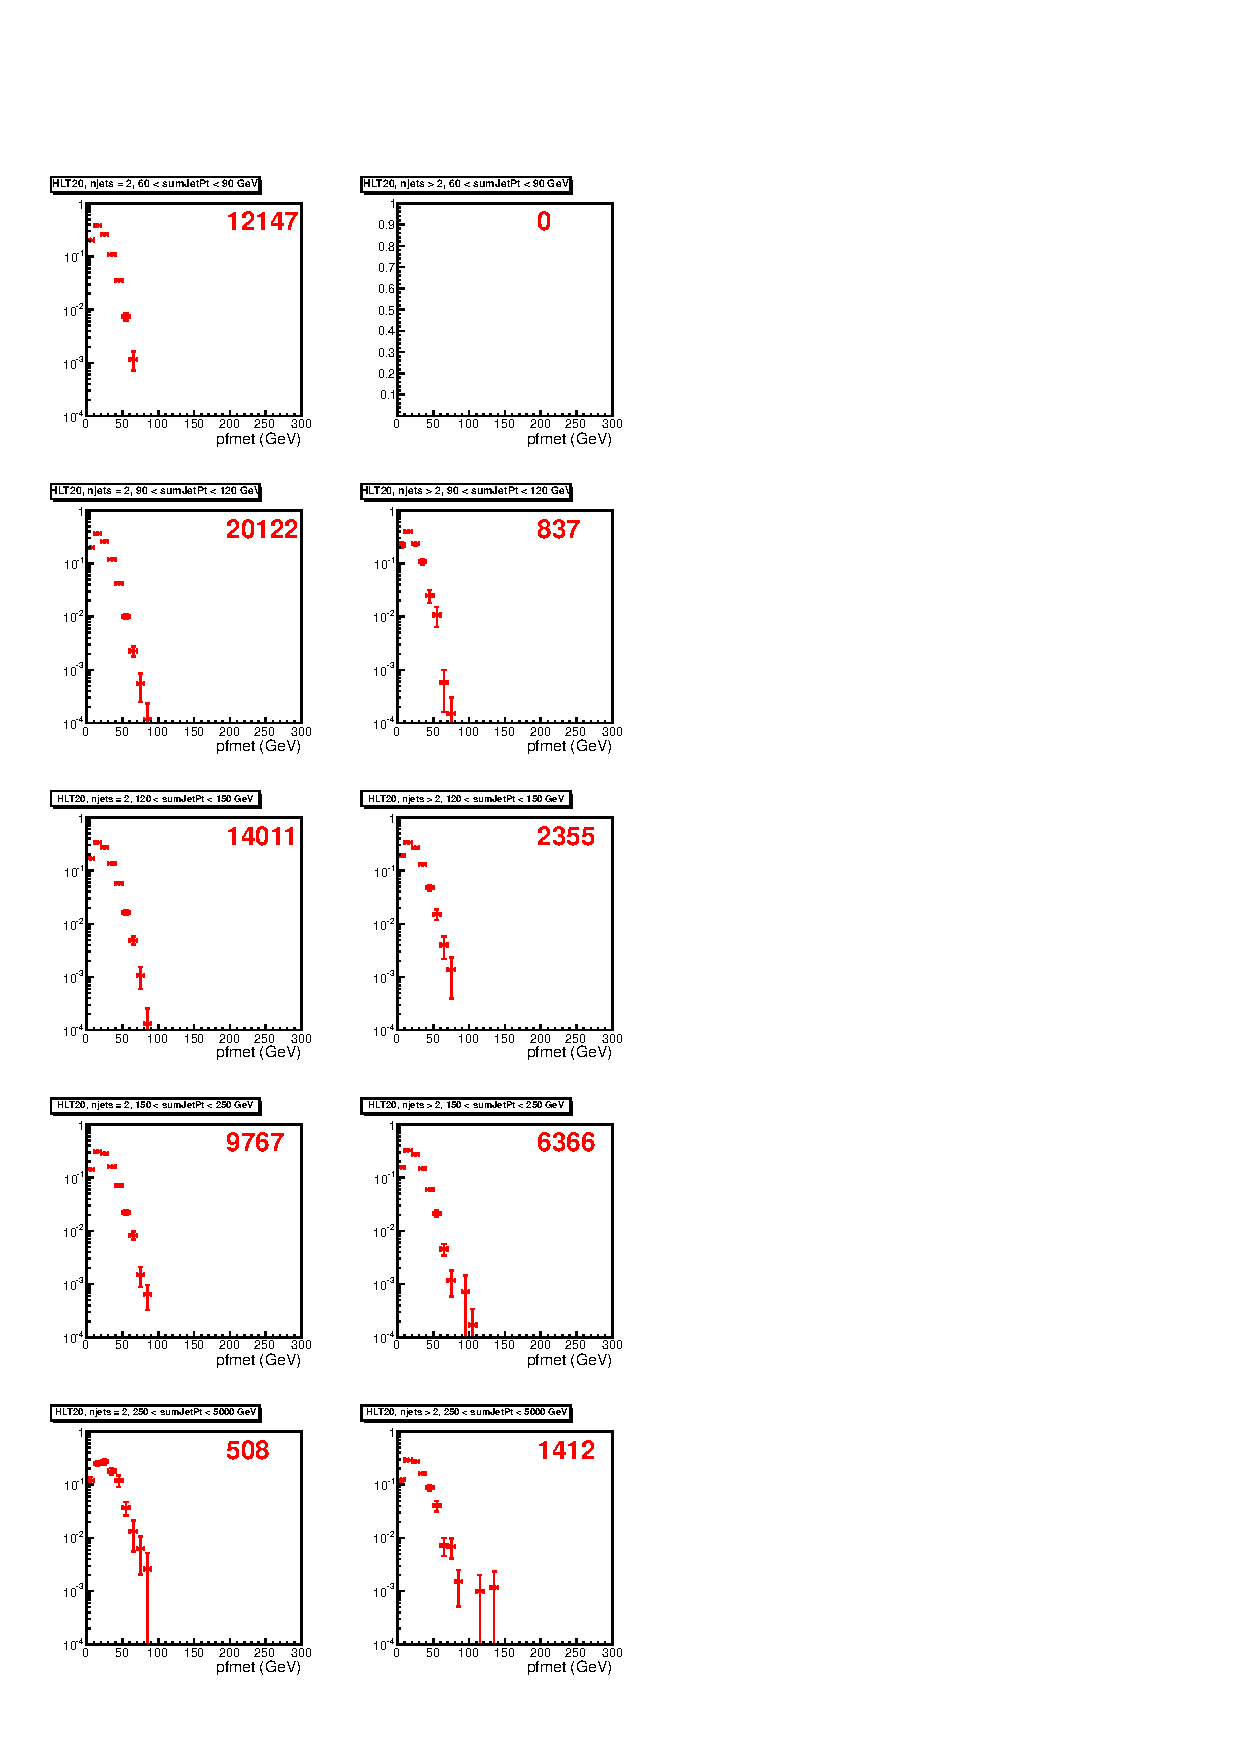
\includegraphics[width=0.5\textwidth]{plots/template_inclusive_0.pdf}
\end{tabular}
\caption{
\MET\ templates for the inclusive analysis collected with the \pt $>$ 22 GeV single photon trigger.
The number in red indicates the number of entries in the template.
}
\end{center}
\end{figure}

\clearpage

\begin{figure}[!h]
\begin{center}
\begin{tabular}{cc}
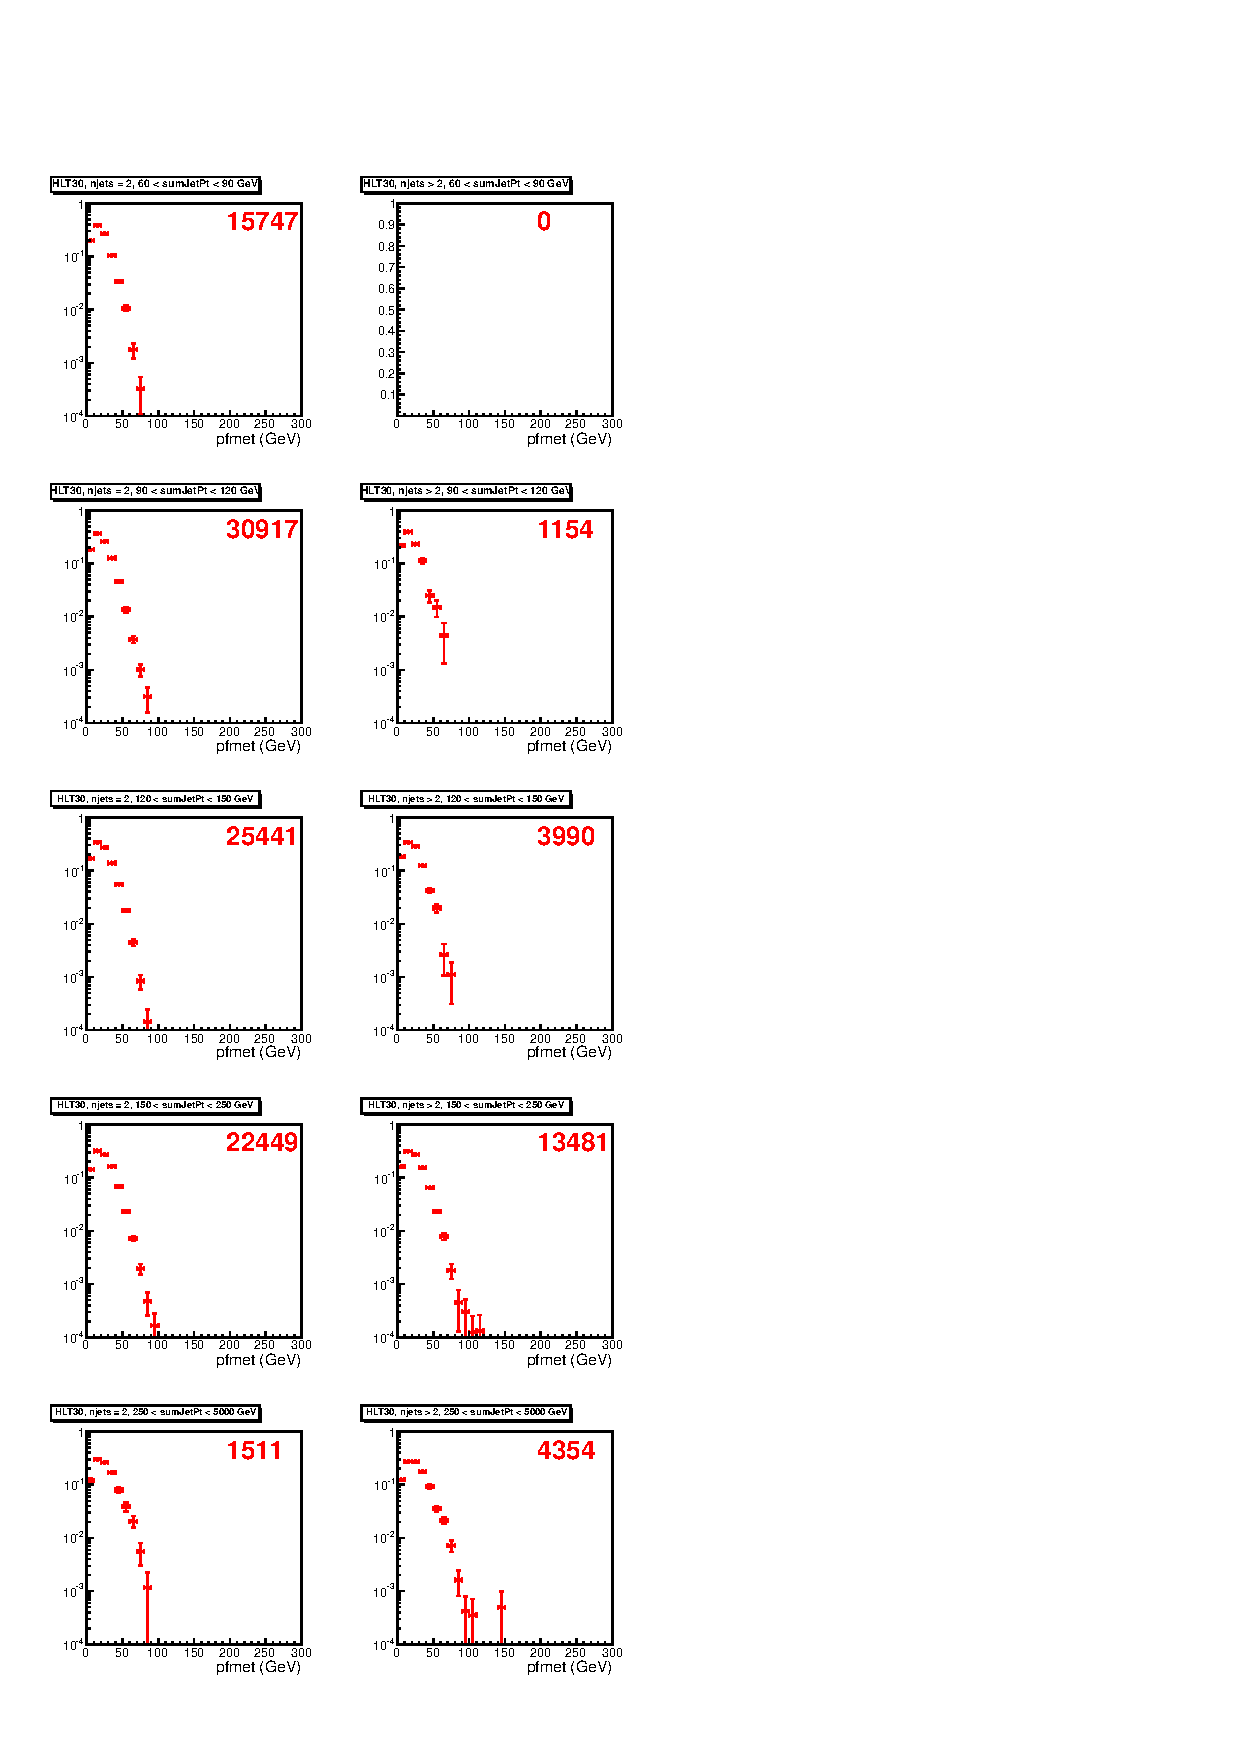
\includegraphics[width=0.5\textwidth]{plots/template_inclusive_1.pdf}
\end{tabular}
\caption{
\MET\ templates for the inclusive analysis collected with the \pt $>$ 36 GeV single photon trigger.
The number in red indicates the number of entries in the template.
}
\end{center}
\end{figure}

\clearpage

\begin{figure}[!h]
\begin{center}
\begin{tabular}{cc}
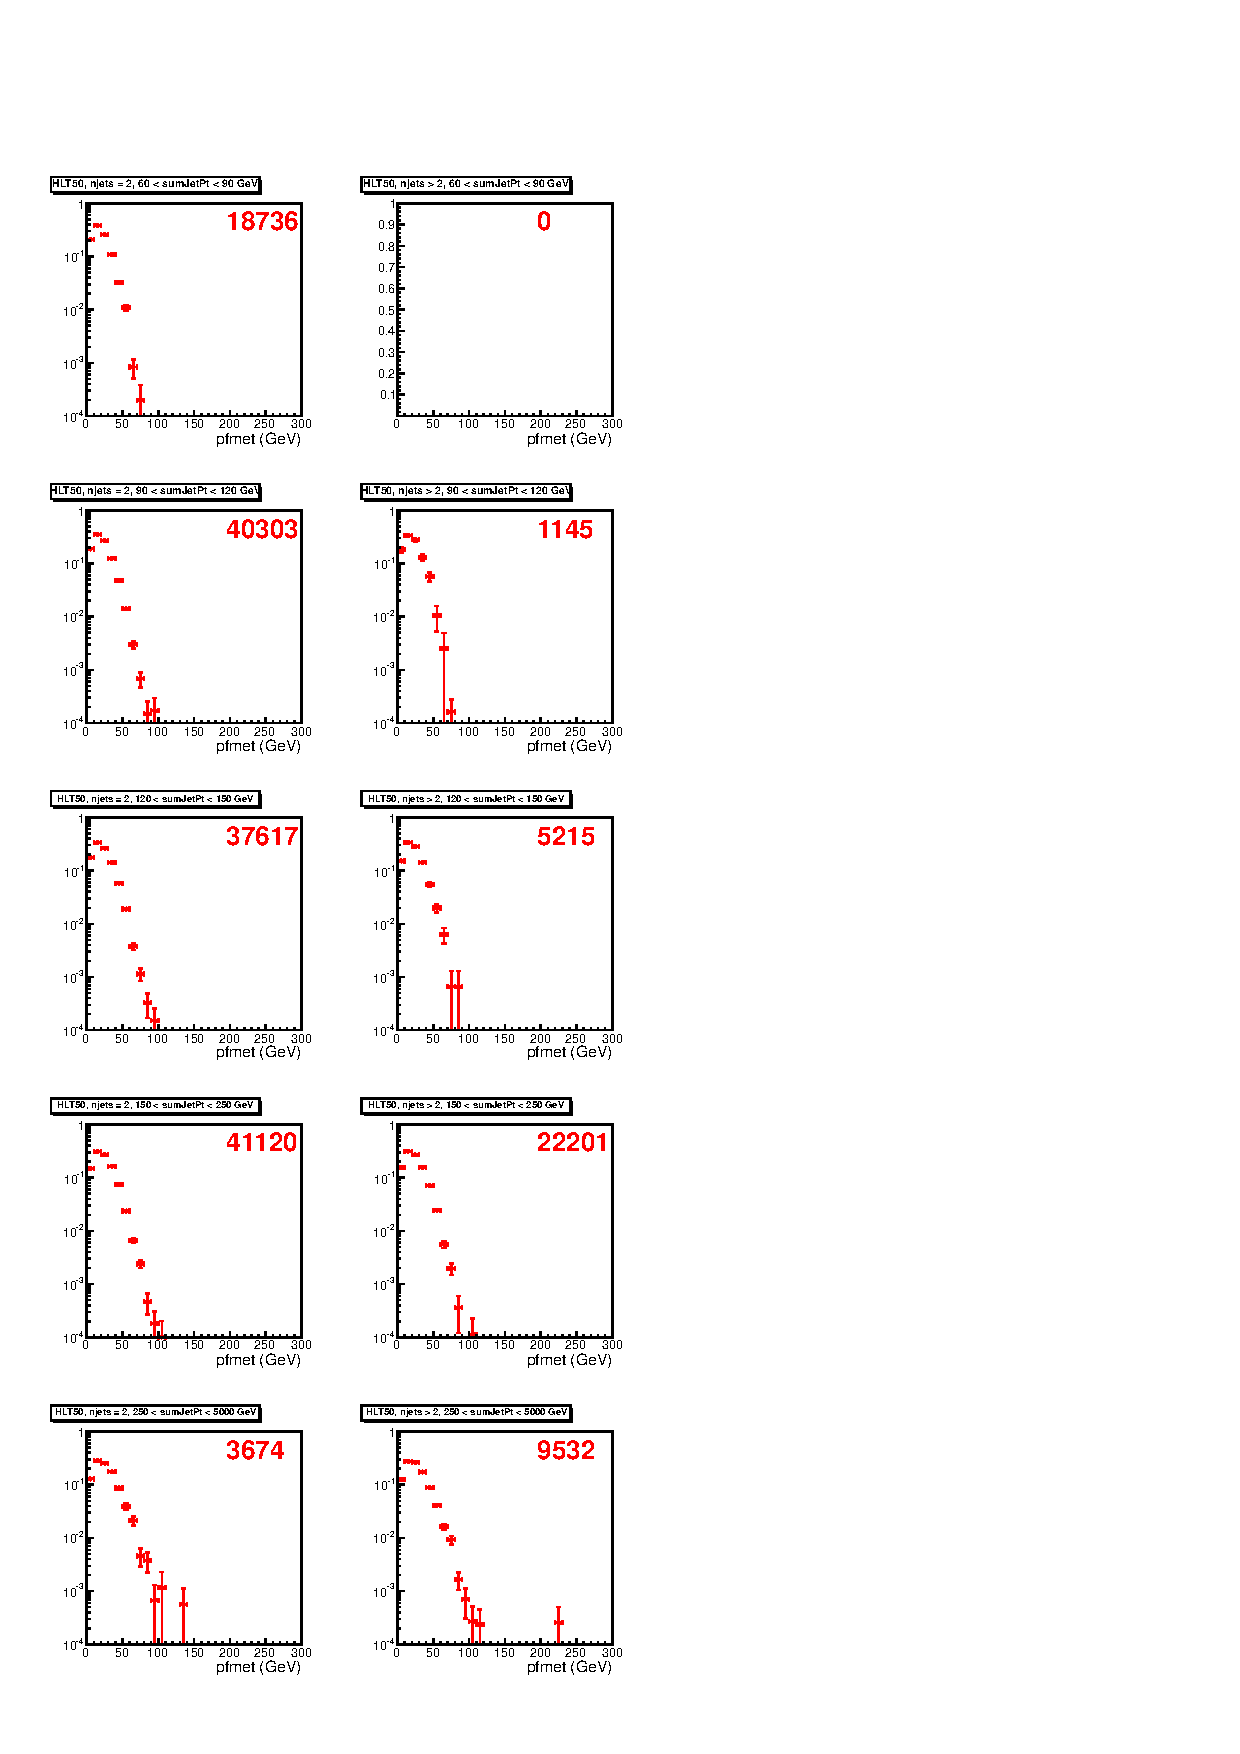
\includegraphics[width=0.5\textwidth]{plots/template_inclusive_2.pdf}
\end{tabular}
\caption{
\MET\ templates for the inclusive analysis collected with the  \pt $>$ 50 GeV single photon trigger.
The number in red indicates the number of entries in the template.
}
\end{center}
\end{figure}

\clearpage

\begin{figure}[!h]
\begin{center}
\begin{tabular}{cc}
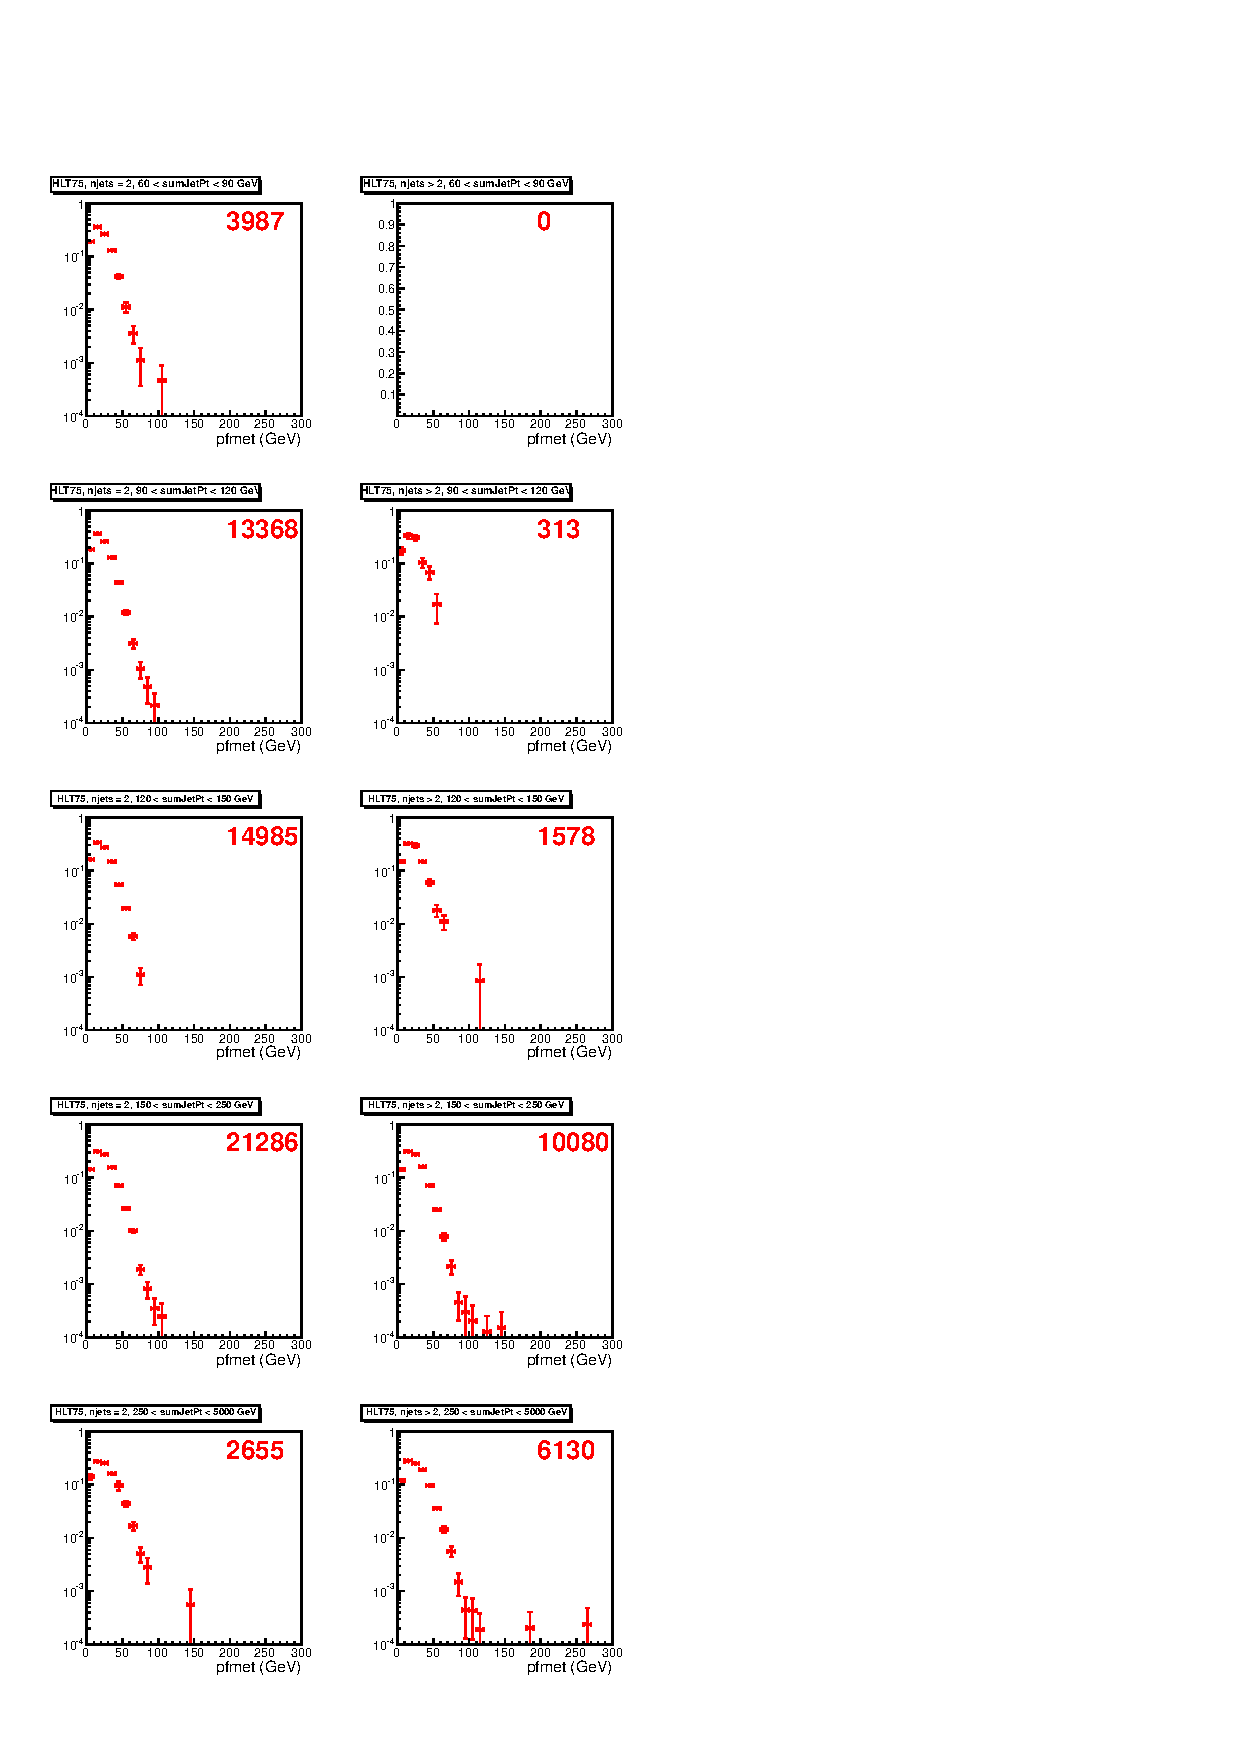
\includegraphics[width=0.5\textwidth]{plots/template_inclusive_3.pdf}
\end{tabular}
\caption{
\MET\ templates for the inclusive analysis collected with the  \pt $>$ 75 GeV single photon trigger.
The number in red indicates the number of entries in the template.
}
\end{center}
\end{figure}

\clearpage

\begin{figure}[!h]
\begin{center}
\begin{tabular}{cc}
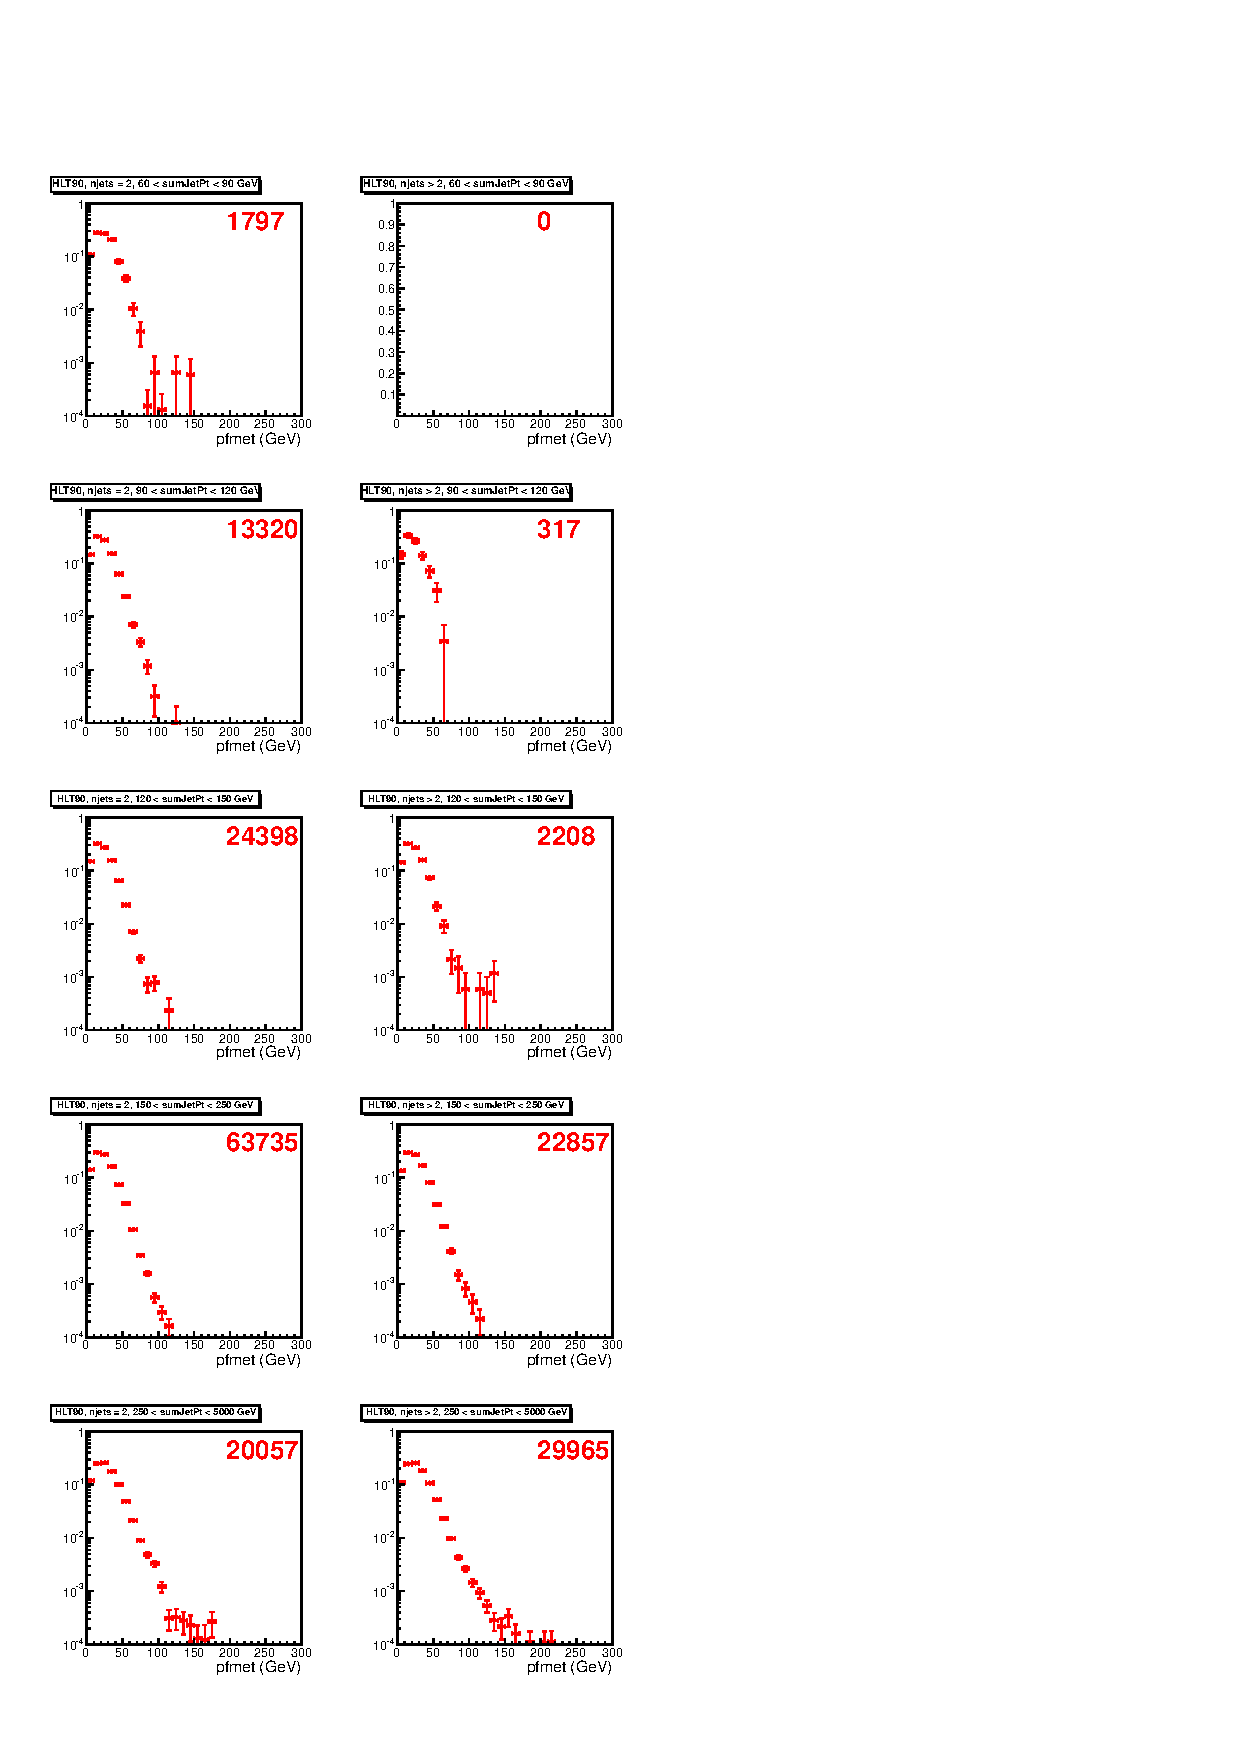
\includegraphics[width=0.5\textwidth]{plots/template_inclusive_4.pdf}
\end{tabular}
\caption{
\MET\ templates for the inclusive analysis collected with the  \pt $>$ 90 GeV single photon trigger.
The number in red indicates the number of entries in the template.
}
\end{center}
\end{figure}

\clearpage

\begin{figure}[!h]
\begin{center}
\begin{tabular}{cc}
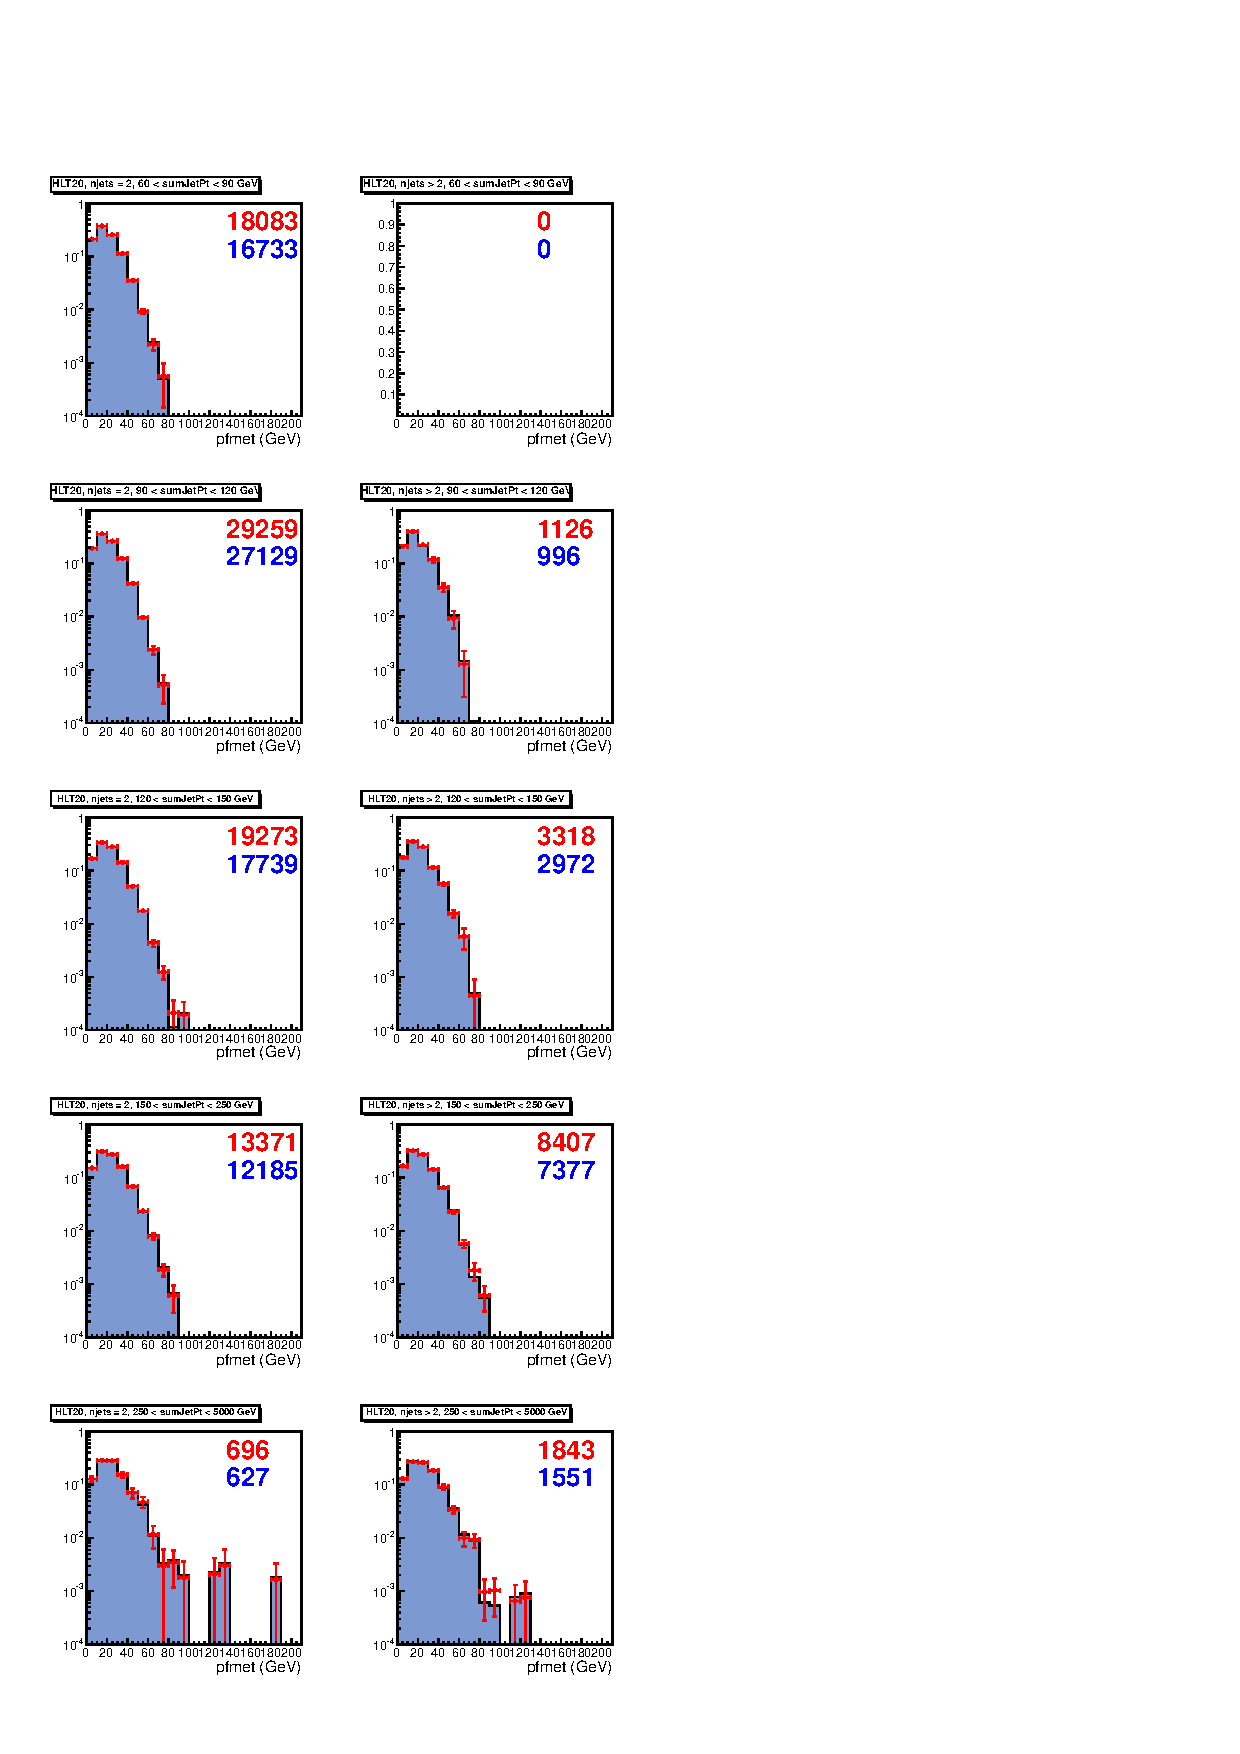
\includegraphics[width=0.5\textwidth]{plots/template_targeted_0.pdf}
\end{tabular}
\caption{
\MET\ templates for the targeted analysis collected with the \pt $>$ 22 GeV single photon trigger.
The number in red indicates the number of entries in the template.
}
\end{center}
\end{figure}

\clearpage

\begin{figure}[!h]
\begin{center}
\begin{tabular}{cc}
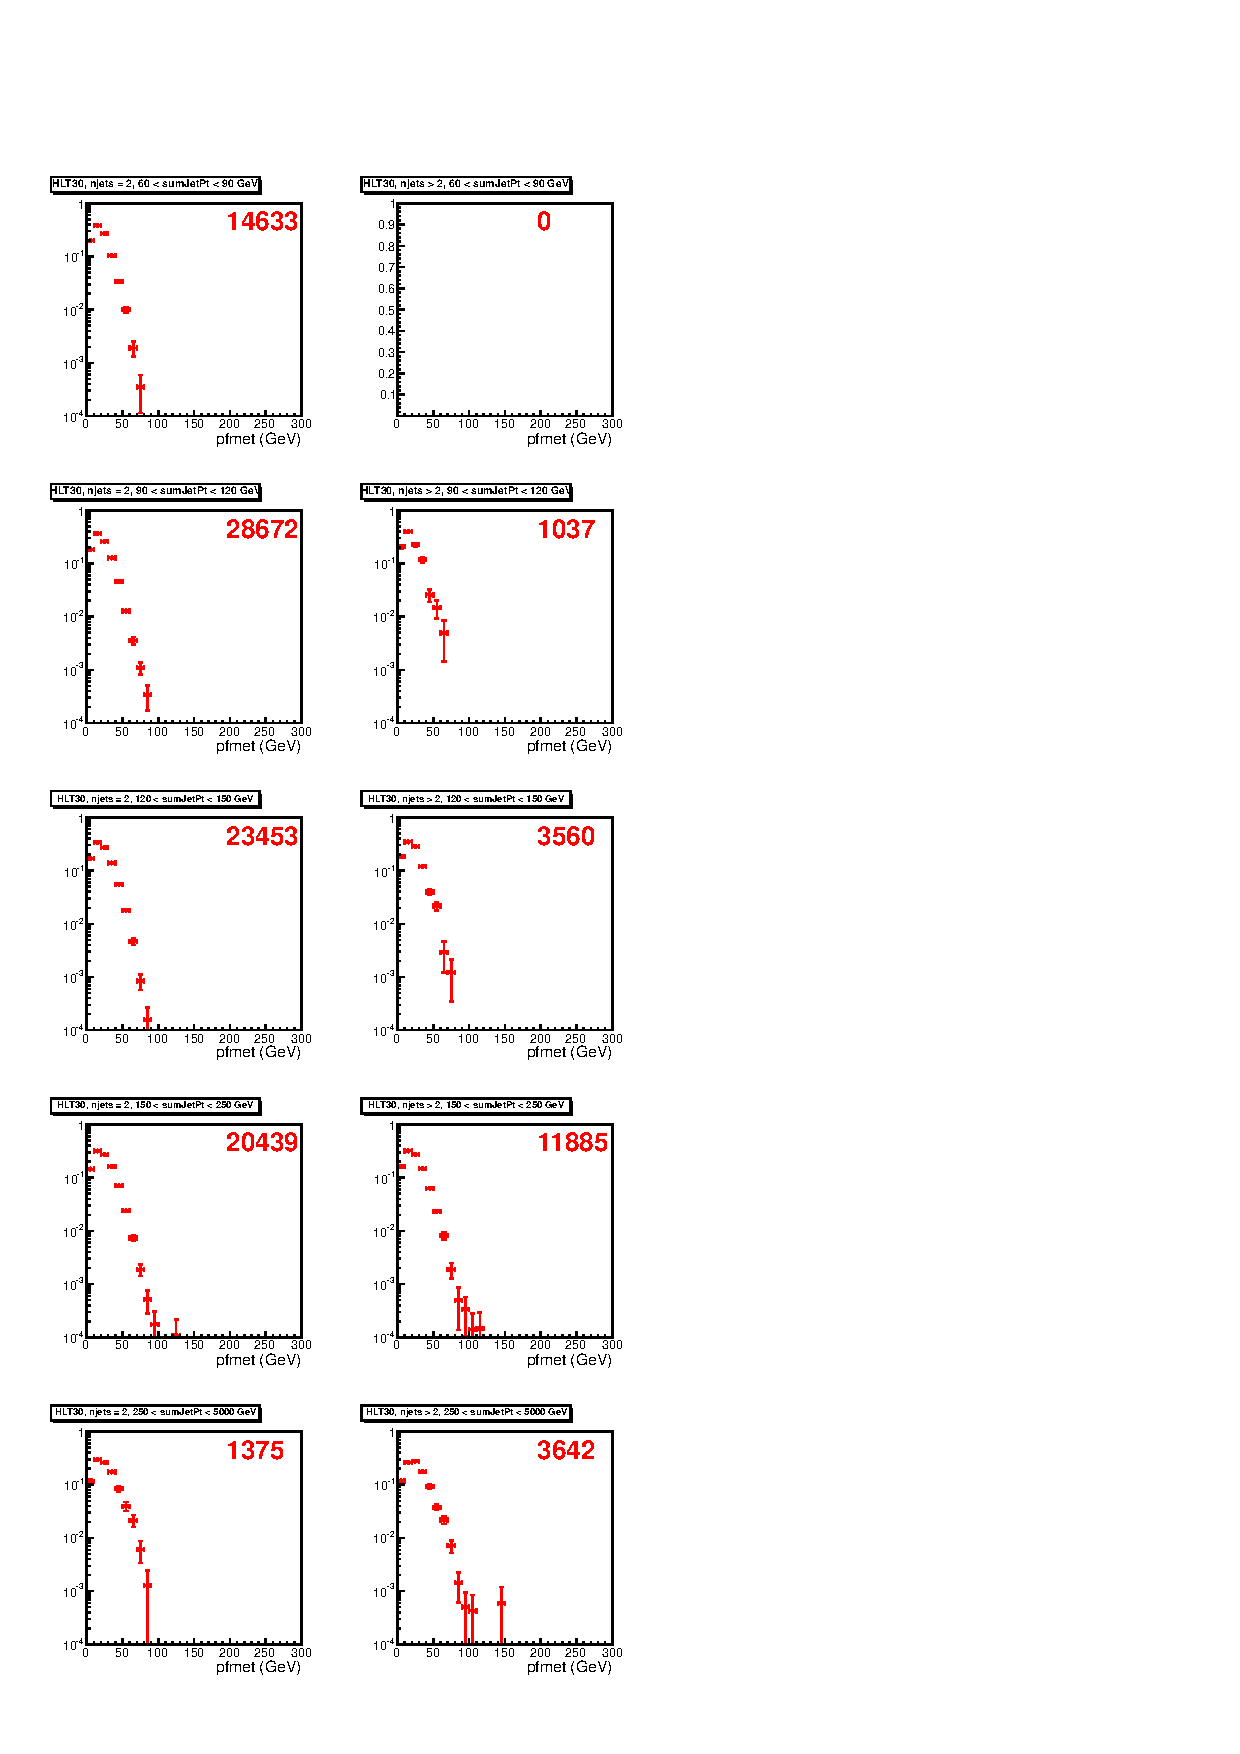
\includegraphics[width=0.5\textwidth]{plots/template_targeted_1.pdf}
\end{tabular}
\caption{
\MET\ templates for the targeted analysis collected with the \pt $>$ 36 GeV single photon trigger.
The number in red indicates the number of entries in the template.
}
\end{center}
\end{figure}

\clearpage

\begin{figure}[!h]
\begin{center}
\begin{tabular}{cc}
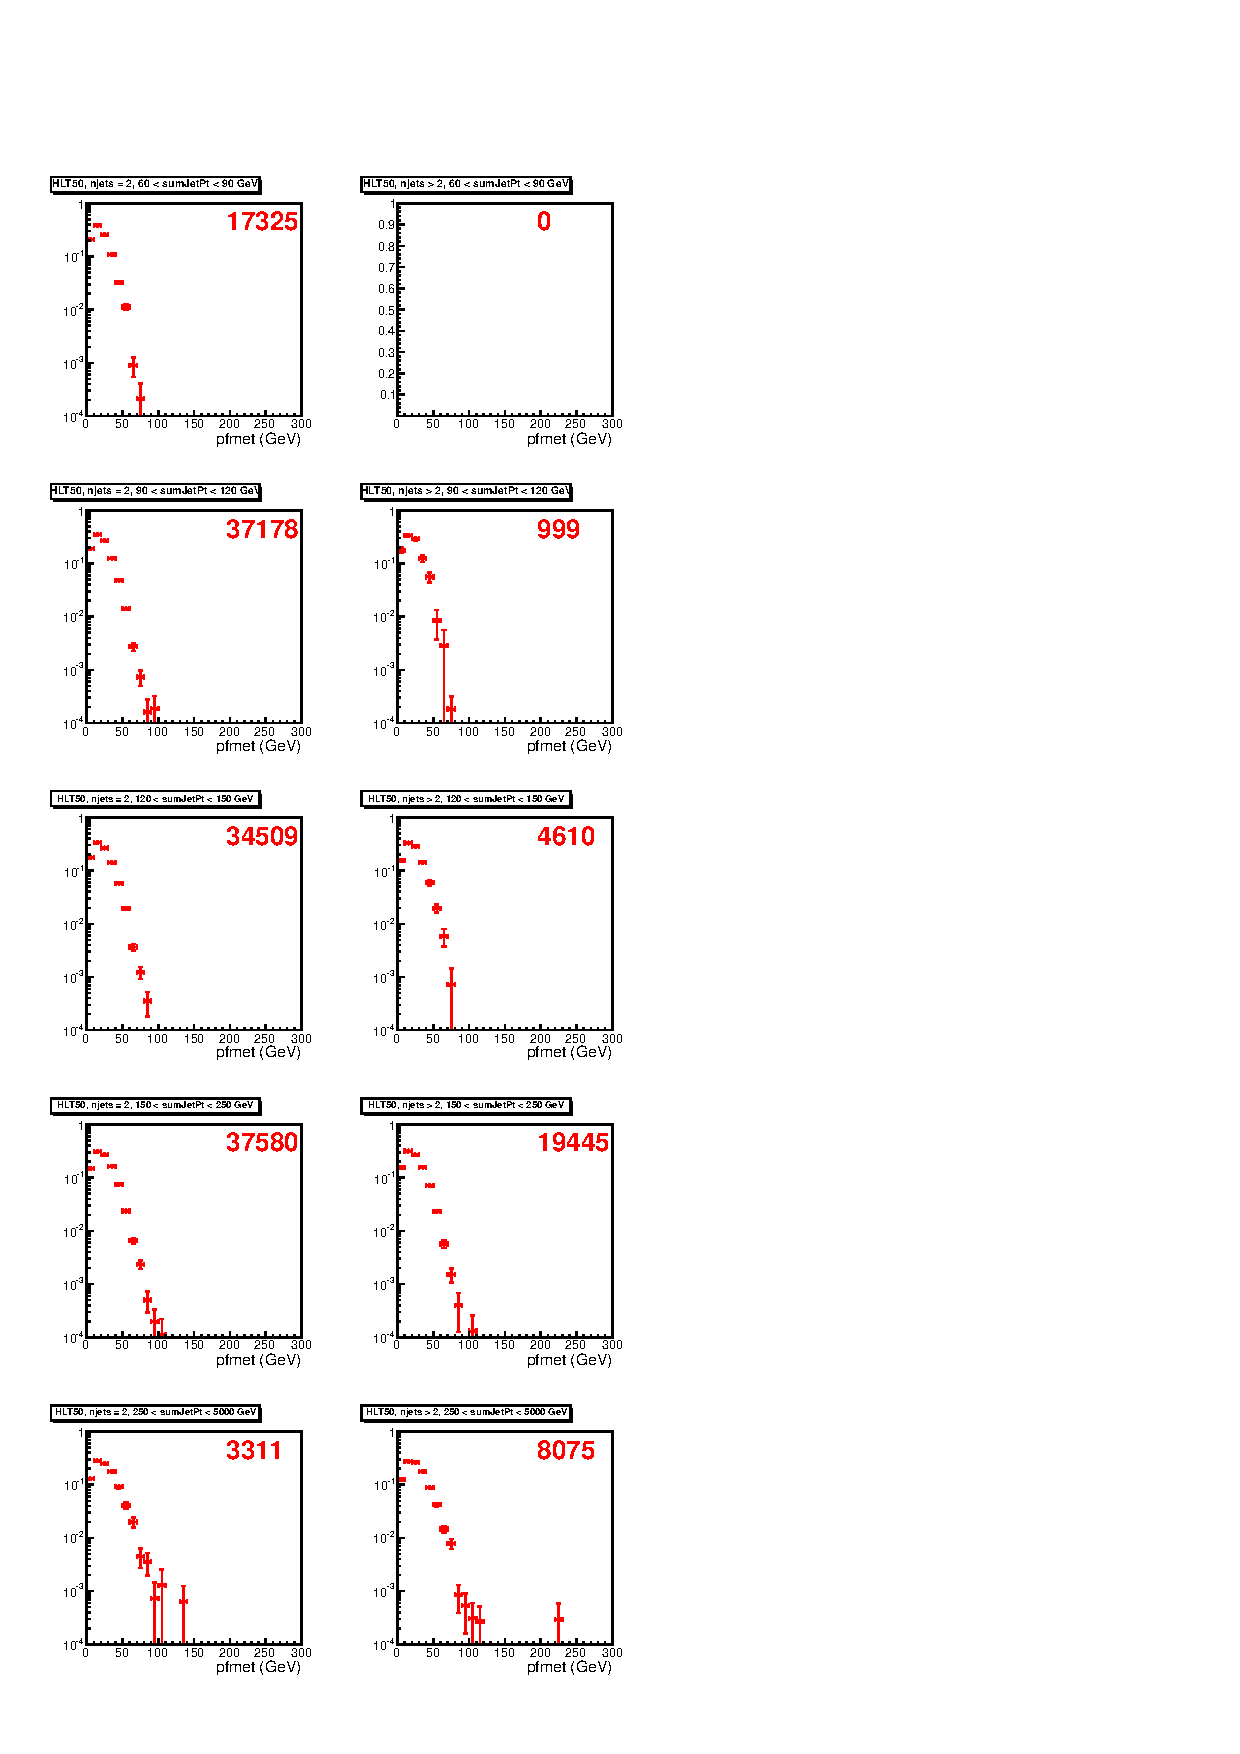
\includegraphics[width=0.5\textwidth]{plots/template_targeted_2.pdf}
\end{tabular}
\caption{
\MET\ templates for the targeted analysis collected with the  \pt $>$ 50 GeV single photon trigger.
The number in red indicates the number of entries in the template.
}
\end{center}
\end{figure}

\clearpage

\begin{figure}[!h]
\begin{center}
\begin{tabular}{cc}
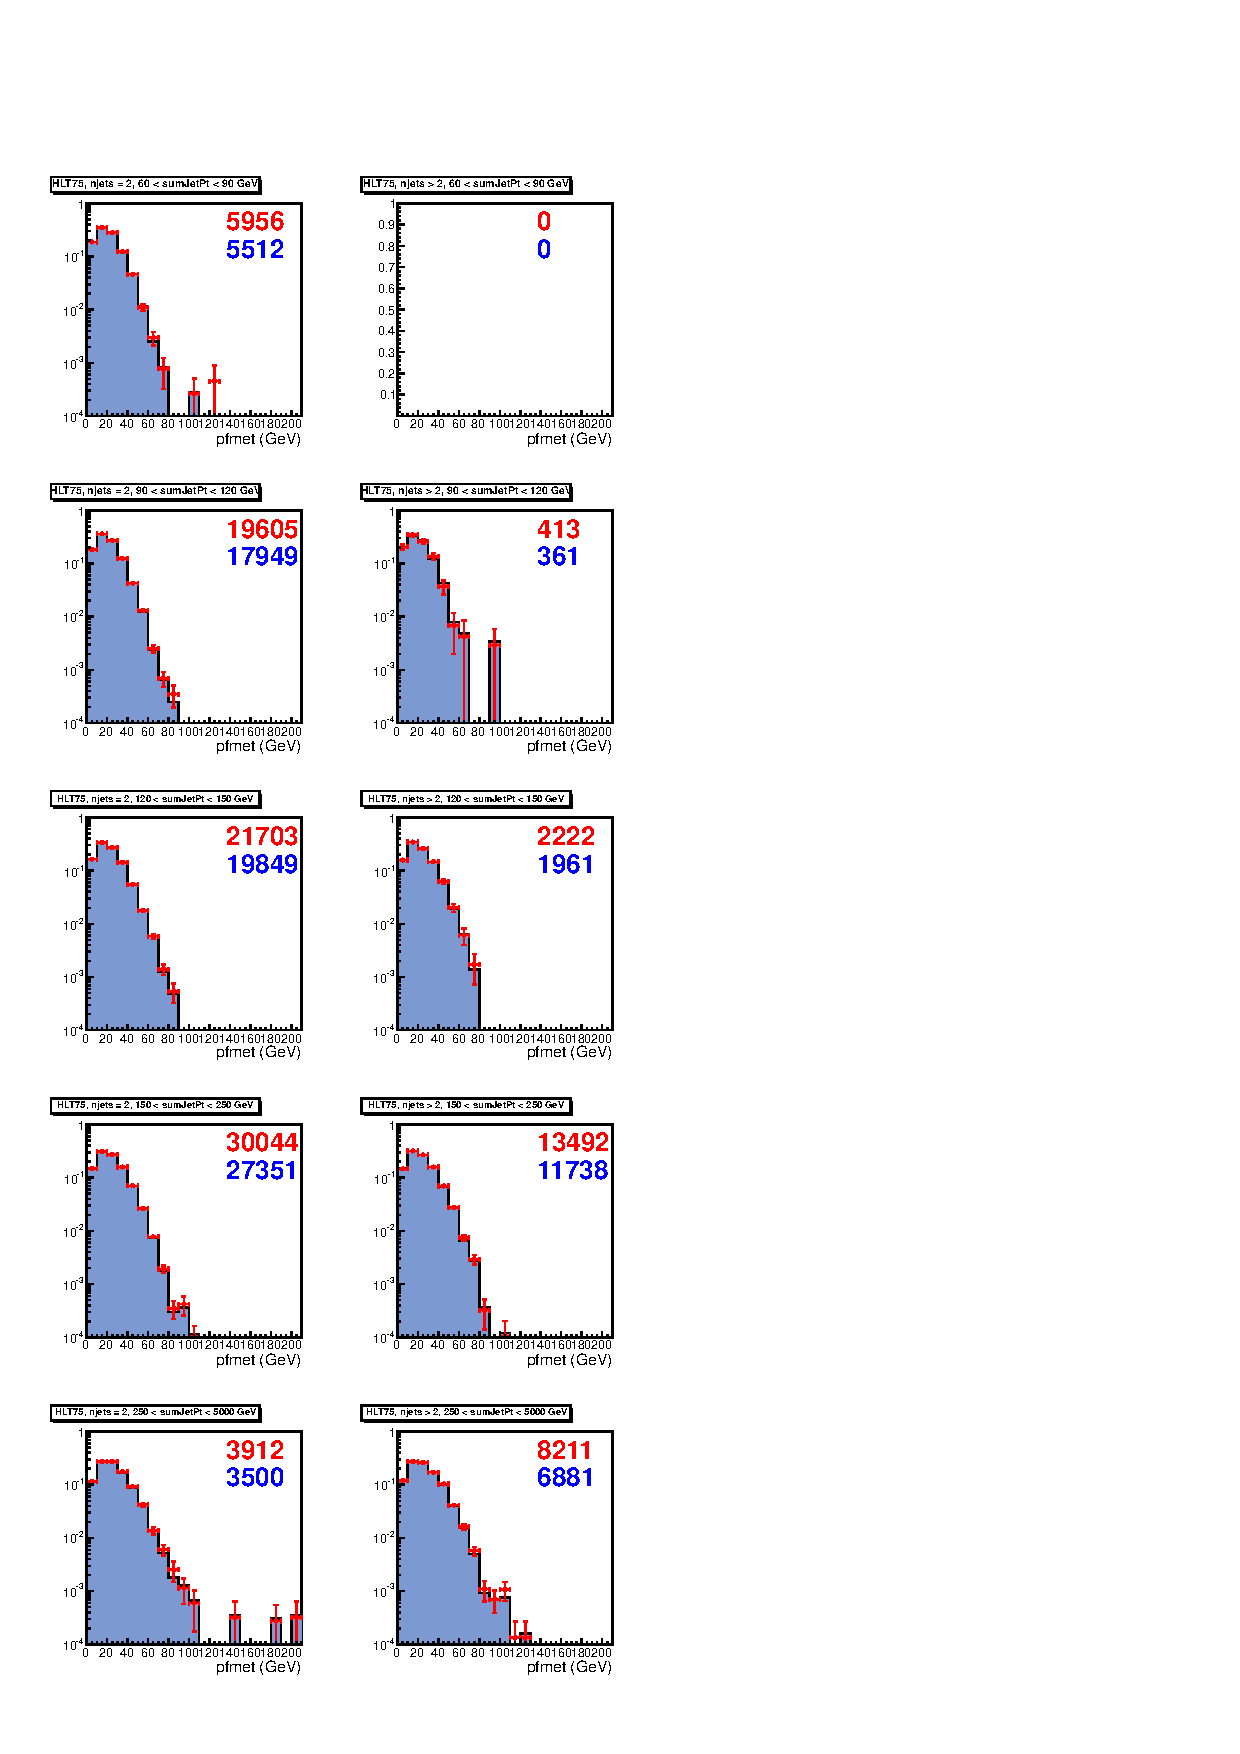
\includegraphics[width=0.5\textwidth]{plots/template_targeted_3.pdf}
\end{tabular}
\caption{
\MET\ templates for the targeted analysis collected with the  \pt $>$ 75 GeV single photon trigger.
The number in red indicates the number of entries in the template.
}
\end{center}
\end{figure}

\clearpage

\begin{figure}[!h]
\begin{center}
\begin{tabular}{cc}
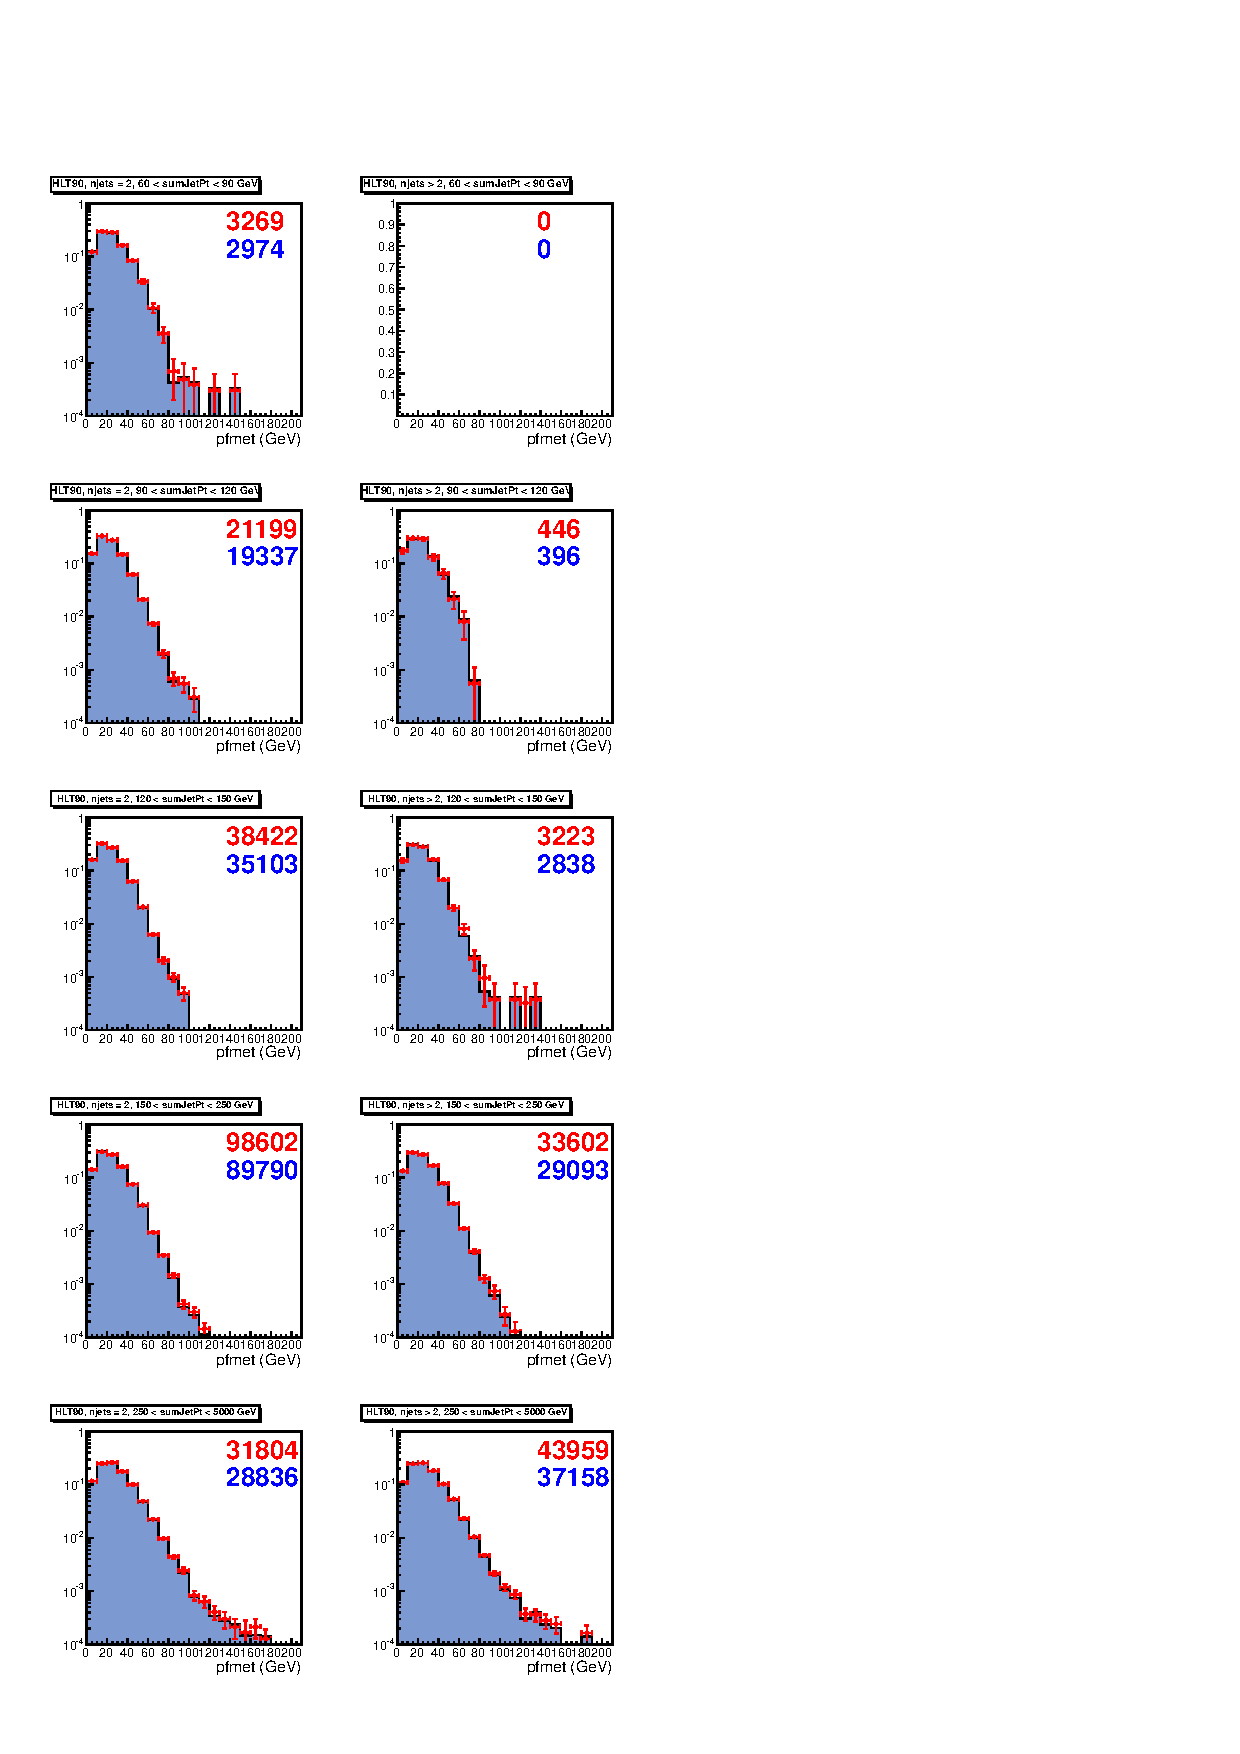
\includegraphics[width=0.5\textwidth]{plots/template_targeted_4.pdf}
\end{tabular}
\caption{
\MET\ templates for the targeted analysis collected with the  \pt $>$ 90 GeV single photon trigger.
The number in red indicates the number of entries in the template.
}
\end{center}
\end{figure}
